
	\citep{asano2008efficient} ont exploité les propriétés du graphe du web pour présenter une nouvelle méthode de compression, appelée 
	\newacronym{ecwg}{ECWG}{Efficient Compression of web graph }	
	\gls{ecwg}, sans perte permettant d'extraire les motifs à partir de la matrice d'adjacence. Ils proposent un vocabulaire composé de six types de blocs (Motifs): un bloc horizontal de 1, un bloc vertical de 1, un bloc diagonal de 1, un rectangle de 1, un bloc de 1 sous forme de L et le singleton 1. Avant de procéder à l'extraction des motifs, la liste d'adjacence du graphe est partitionnée selon les domaines (ex: esi.dz, usthb.dz, ...). Une nouvelle matrice d'adjacence est donc construite pour chaque hôte(domaine) contenant les liens existants entre ses pages, auxquels les liens inter-hôtes sont concaténés.
					Les blocs B sont détectés par la suite et chacun est représenté par un quadruplets (i, j, type(B), dim(B)) où i,j représentent les coordonnées du premier élément du bloc dans la matrice d'adjacence de l'hôte, type(B) représente le type du bloc et dim(B) représente les dimensions du bloc (omis dans le cas du singleton). 
					\begin{figure}[h]
					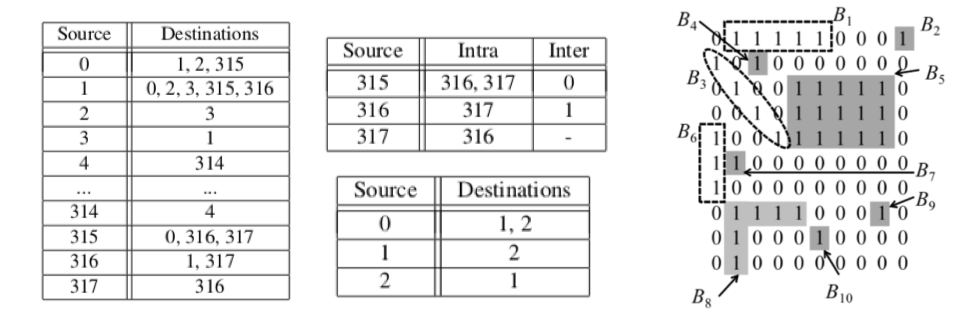
\includegraphics[scale=0.5]{ressources/image/inter_intra.png} 
					\caption{Exemple illustrant le principe de fonctionnement \citep{asano2008efficient}}
					\label{interIntra}
				\end{figure}